\documentclass[presentation]{beamer}

\usepackage{tikz}
\usetikzlibrary{positioning,calc}
\usetikzlibrary{shapes.geometric}
\usetikzlibrary{backgrounds}% only to show the bounding box
\usetikzlibrary{shapes,arrows}
\usepackage{pgfplots}
\usepackage{pgfplotstable}
\usetikzlibrary{pgfplots.groupplots}
\pgfplotsset{compat=1.12}
\usepackage{appendixnumberbeamer}
\usepackage{amsmath}
\date{26th January 2017}
\usetheme{firedrake

\pgfplotscreateplotcyclelist{decent cycle}{%
  {blue, mark=*, mark options={fill=blue},
    mark size=2pt},
  {cyan, mark=square*, mark options={fill=cyan},
    mark size=2pt},
  {magenta, mark=triangle*, mark options={fill=magenta},
    mark size=3pt},
  {blue, mark=*, mark options={fill=blue},
    mark size=2pt},
  {cyan, mark=square*, mark options={fill=cyan},
    mark size=2pt},
  {magenta, mark=triangle*, mark options={fill=magenta},
    mark size=3pt},
}

\pgfplotsset{
  decent/.style={
    cycle list name=decent cycle,
  }
}
\renewcommand{\vec}[1]{\ensuremath{\boldsymbol{#1}}}
\newcommand{\ddt}[1]{\frac{\partial #1}{\partial t}}
\newcommand{\zhat}{\hat{\vec{z}}}
\newcommand{\W}{\ensuremath{\mathbb{W}}}

\DeclareMathOperator{\grad}{grad}
\let\div\relax
\DeclareMathOperator{\div}{div}
\DeclareMathOperator{\curl}{curl}
\newcommand{\vsubset}[1]{\rotatebox[origin=c]{90}{\ensuremath{\subset}}}
\newcommand{\inner}[2]{\ensuremath{\langle #1, #2 \rangle}}
\author{Lawrence Mitchell\inst{1}}
\institute{
\inst{1}Departments of Computing and Mathematics, Imperial College
London
}

\graphicspath{{./\jobname.figures/}}

\newcommand{\arxivlink}[2]{%
  \href{http://www.arxiv.org/abs/#1}%
  {{\small\texttt{arXiv:\,#1\,[#2]}}}%
}
\newcommand{\doilink}[1]{%
  \href{http://dx.doi.org/#1}%
  {{\small\texttt{doi:\,#1}{}}}%
}
\usepackage[url=false,
            doi=true,
            isbn=false,
            style=authoryear,
            firstinits=true,
            uniquename=init,
            backend=biber]{biblatex}

\setbeamertemplate{bibliography item}{}
\renewcommand{\bibfont}{\footnotesize}
\addbibresource{references.bib}

\setlength{\bibitemsep}{1ex}

\renewbibmacro{in:}{}
\DeclareFieldFormat[article]{volume}{\textbf{#1}}
\DeclareFieldFormat{doi}{%
  doi\addcolon%
  {\scriptsize\ifhyperref{\href{http://dx.doi.org/#1}{\nolinkurl{#1}}}
    {\nolinkurl{#1}}}}
\AtEveryBibitem{%
\clearfield{pages}%
\clearfield{issue}%
\clearfield{number}%
}

\usepackage{minted}

\title{Firedrake: automating the finite element method by composing
  abstractions}

\begin{document}

\maketitle

\begin{frame}
  \frametitle{Firedrake team}
  \begin{itemize}
  \item[IC] Thomas Gibson, David A.~Ham, Mikl\'os Homolya, {\color{gray}Fabio
    Luporini}, Tianjiao Sun, Paul H.~J.~Kelly
  \item[Bath] Andrew T.~T.~McRae
  \item[\color{gray}ECMWF] \color{gray}Florian Rathgeber
  \item[\color{gray}IBM] \color{gray}Gheorghe-Teodor Bercea
  \end{itemize}
  \begin{center}
    \url{www.firedrakeproject.org}\\
    \cite{Rathgeber:2016} \arxivlink{1501.01809}{cs.MS}
  \end{center}
\end{frame}

\begin{frame}
  \frametitle{Contact}

  \begin{center}
    \large
    \url{www.firedrakeproject.org/contact.html}
  \end{center}
  \begin{block}{Methods}
    \begin{itemize}
    \item Slack: \url{firedrakeproject.slack.com}
    \item Mail: \texttt{firedrake@imperial.ac.uk} (subscribe first)
    \item Github: \url{github.com/firedrakeproject/firedrake}
    \end{itemize}
  \end{block}
\end{frame}

\begin{frame}
  \frametitle{What is Firedrake?}
  \begin{quote}
    {\normalfont [\ldots]} an automated system for the portable solution of partial
    differential equations using the finite element method.
  \end{quote}

  \begin{itemize}
  \item Written in Python.
  \item Finite element problems specified with \emph{embedded} domain
    specific language.
  \item \emph{Runtime} compilation to low-level (C) code.
  \item Expressly \emph{data parallel}: don't worry about MPI.
  \end{itemize}
\end{frame}

\begin{frame}[fragile]
  \frametitle{A specification of finite element problems}
  \begin{columns}
    \begin{column}[t]{0.65\textwidth}
\begin{minted}[fontsize=\tiny]{python}
from firedrake import *
mesh = UnitSquareMesh(100, 100)
V = FunctionSpace(mesh, "RT", 2)
Q = FunctionSpace(mesh, "DG", 1)
W = V*Q
u, p = TrialFunctions(W)
v, q = TestFunctions(W)

a = dot(u, v)*dx + div(v)*p*dx + div(u)*q*dx
L = -Constant(1)*v*dx
u = Function(W)
solve(a == L, u, solver_parameters={
    "ksp_type": "gmres", 
    "ksp_rtol": 1e-8,
    "pc_type": "fieldsplit",
    "pc_fieldsplit_type": "schur",
    "pc_fieldsplit_schur_fact_type": "full",
    "pc_fieldsplit_schur_precondition": "selfp",
    "fieldsplit_0_ksp_type": "preonly",
    "fieldsplit_0_pc_type": "ilu",
    "fieldsplit_1_ksp_type": "preonly",
    "fieldsplit_1_pc_type": "hypre"
})
\end{minted}
    \end{column}
    \hspace{-4em}
    \begin{column}[t]{0.5\textwidth}
      Find $u\in V\times Q\subset H(\div)\times L^2$ s.t.
      \begin{align*}
        \inner{u}{v} + \inner{\div v}{p} &= 0 \quad\forall\, v \in V\\
        \inner{\div u}{q} &= -\inner{1}{q}\quad\forall\, q \in Q.
      \end{align*}
    \end{column}
  \end{columns}
\end{frame}


\begin{frame}[fragile]
  \frametitle{Symbolic, numerical computing}
  Weave together
  \begin{itemize}
  \item \emph{symbolic} problem description
\begin{minted}[fontsize=\tiny]{python}
W = V*Q
u, p = TrialFunctions(W)
v, q = TestFunctions(W)
a = dot(u, v)*dx + div(v)*p*dx + div(u)*q*dx
L = -Constant(1)*v*dx
\end{minted}
  \item with problem-specific data (which mesh, what solver?)
\begin{minted}[fontsize=\tiny]{python}
mesh = UnitSquareMesh(100, 100)
V = FunctionSpace(mesh, "RT", 2)
Q = FunctionSpace(mesh, "DG", 1)
...
solve(a == L, u, solver_parameters=...)
\end{minted}
  \end{itemize}
  and \emph{synthesise} efficient implementation from
  the symbolic problem description.
\end{frame}
\begin{frame}
  \frametitle{More than a pretty face}

  \begin{block}{Library usability}
    \begin{itemize}
    \item High-level language enables rapid model development
    \item Ease of experimentation
    \item Small model code base
    \end{itemize}
  \end{block}

  \begin{block}{Library development}
    \begin{itemize}
    \item Automation of complex optimisations
    \item Exploit expertise across disciplines
    \item Small library code base
    \end{itemize}
  \end{block}
\end{frame}

\begin{frame}[fragile]
  \frametitle{Composability of libraries that manipulate PDE solvers}
  \begin{block}{\url{www.dolfin-adjoint.org}}
    Automated derivation of the discrete adjoint from forward models
    written using FEniCS \emph{and Firedrake}.

\begin{minted}[fontsize=\scriptsize]{sh}
$ cloc dolfin-adjoint/
Language  files   blank   comment   code
Python       54    2322       937   7294
$ cloc dolfin-adjoint/compatibility.py
Python        1      38        11    140
\end{minted}
  \end{block}
\end{frame}

\begin{frame}
  \frametitle{Ease of experimentation}
  How much code do you need to change to
  \begin{itemize}
  \item Change preconditioner (e.g.~ILU to AMG)?
  \item Drop terms in the preconditioning operator?
  \item Use a completely different operator to precondition?
  \item Do quasi-Newton with an approximate Jacobian?
  \item Apply operators matrix-free?
  \end{itemize}

  Same ``easy to use'' code must run fast at scale.
\end{frame}

\begin{frame}[standout]
  Say \emph{what}, not \emph{how}.
\end{frame}

\begin{frame}
  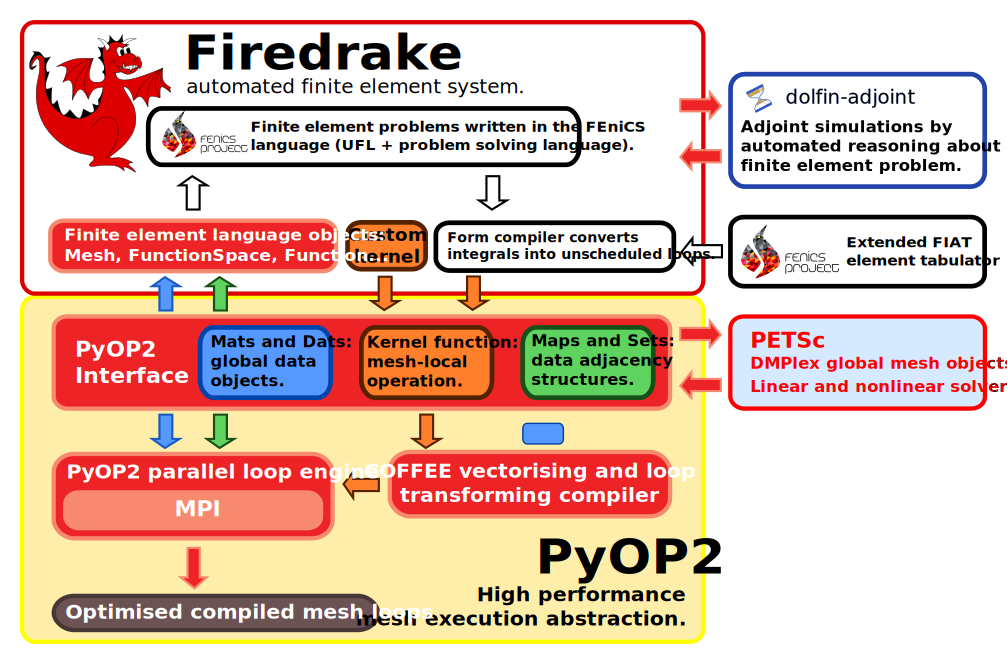
\includegraphics[width=\textwidth]{firedrake-stack}
\end{frame}

\section{Local kernels}

\begin{frame}
  \frametitle{Automating expertise}
  \begin{itemize}
  \item ``In-person'' case-by-case optimisation \emph{does not scale}
  \item Code generation allows us to package expertise and provide it
    to everyone
  \item Done by a special-purpose kernel compiler
  \end{itemize}
\end{frame}

\begin{frame}[allowframebreaks]
  \frametitle{COFFEE}

  No single optimal schedule for evaluation of every finite element
  kernel.  Variability in
  \begin{itemize}
  \item polynomial degree,
  \item number of fields,
  \item kernel complexity,
  \item working set size,
  \item structure in the basis functions,
  \item structure in the quadrature points,
  \item ...
  \end{itemize}

\pagebreak

\begin{block}{Vectorisation}
  Align and pad data structures, then use intrinsics or rely on
  compiler.\\
  \cite{Luporini:2015} \doilink{10.1145/2687415}
\end{block}

\begin{block}{Flop reduction}
  Exploit \emph{linearity} in test functions to perform factorisation,
  code motion and CSE.  

  \cite{Luporini:2016} \arxivlink{1604.05872}{cs.MS}
\end{block}

\begin{center}
  \url{github.com/coneoproject/COFFEE}
\end{center}
\end{frame}

\section{Global iteration}

\begin{frame}[allowframebreaks]
  \frametitle{Tensions in model development}

  \begin{block}{Performance}
    \begin{itemize}
    \item Keep data in cache as long as possible.  
    \item Manually fuse kernels.
    \item Loop tiling for latency hiding.
    \item ...
    \item Individual components hard to test
    \item Space of optimisations suffers from combinatorial
      explosion.
    \end{itemize}
  \end{block}

\pagebreak
  \begin{block}{Maintainability}
    \begin{itemize}
    \item Keep kernels separate
    \item ``Straight-line'' code
    \item ...
    \item Testable
    \item Even if performance of individual kernels is good, can lose
      \emph{a lot}
    \end{itemize}
  \end{block}

\end{frame}

\begin{frame}[fragile]
  \frametitle{PyOP2}
  A library for expressing data parallel iterations
\begin{description}
\item[{\emph{Sets}}] iterable entities
\item[{\emph{Dats}}] abstract managed arrays (data defined on a set)
\item[{\emph{Maps}}] relationships between elements of sets
\item[{\emph{Kernels}}] local computation
\item[{\emph{par\_loop}}] Data parallel iteration over a set
\end{description}
Arguments to parallel loop indicate how to gather/scatter global
data using \emph{access descriptors}

\begin{minted}[fontsize=\scriptsize]{python}
par_loop(kernel, iterset, data1(map1, READ), data2(map2, WRITE))
\end{minted}
\end{frame}

\begin{frame}
  \frametitle{Key ideas}
  \begin{block}{Local computation}
    Kernels do not know about global data layout.
    \begin{itemize}
    \item Kernel defines contract on local, packed, ordering.
    \item Global-to-local reordering/packing appears in map.
    \end{itemize}
  \end{block}
  \begin{block}{``Implicit'' iteration}
    Application code does not specify explicit iteration order.
    \begin{itemize}
    \item Define data structures, then just ``iterate''
    \item Lazy evaluation
    \end{itemize}
  \end{block}
\end{frame}

\section{Did we succeed?}

\begin{frame}
  \frametitle{Experimentation}
  
  With model set up, experimentation is easy

  \begin{itemize}
  \item Change preconditioner: c. 1 line
  \item Drop terms: c. 1-4 lines
  \item Different operator: c. 1-10 lines
  \item quasi-Newton: c. 1-10 lines
  \item Matrix-free: c. 1-10 lines (+ c. 30 lines for preconditioner).
  \end{itemize}
\end{frame}

\begin{frame}
  \frametitle{Maintainability}
  \begin{columns}
    \begin{column}[t]{0.5\textwidth}
      \begin{block}{Core Firedrake}
        \begin{table}
          \centering
          \begin{tabular}{lc}
            Component & LOC \\
            \hline
            Firedrake & 11000 \\
            PyOP2     & 5000 \\
            TSFC      & 3500 \\
            COFFEE    & 4500 \\
            \hline
            Total     & 24000
          \end{tabular}
        \end{table}
      \end{block}
    \end{column}
    \begin{column}[t]{0.5\textwidth}
      \begin{block}{Shared with FEniCS}
        \begin{table}
          \centering
          \begin{tabular}{lc}
            Component & LOC \\
            \hline
            FIAT & 4000 \\
            UFL     & 13000 \\
            \hline
            Total & 17000
          \end{tabular}
        \end{table}        
      \end{block}
    \end{column}
  \end{columns}
\end{frame}
\begin{frame}[allowframebreaks]
  \frametitle{Performance}

  \begin{block}{Kernel performance}
    \begin{itemize}
    \item COFFEE produces kernels that are better (operation count)
      than existing automated form compilers
    \item Provably optimal in some cases
    \item Good vectorised performance, problem dependent, but up to
      70\% peak for in-cache computation.
    \end{itemize}
  \end{block}

\end{frame}

\begin{frame}
  \frametitle{Summary}
  \begin{itemize}
  \item Firedrake provides a layered set of abstractions for finite
    element
  \item Enables automated provision of expertise to model developers
  \item Computational performance is good, often $>50\%$ achievable
    peak.
  \end{itemize}
\end{frame}

\appendix
\begin{frame}[t]
  \frametitle{References}
  \printbibliography[heading=none]
\end{frame}
\end{document}
